\section{System Design}
		\vs
		To solve actual problems in an industry setting, a software engineer or a team of Engineers must incorporate a development strategy that encompasses the process, methods, and tools layers. This strategy is often referred to as a process model or a software engineering paradigm. A process model or a software engineering is chosen based on the nature of the project and application, the methods and tools to be used, and the controls and deliverables that are required.
		\vs
		In this project, \textbf{\em Waterfall Model} is used which involve steps given below:
		\vs
		\begin{center}
			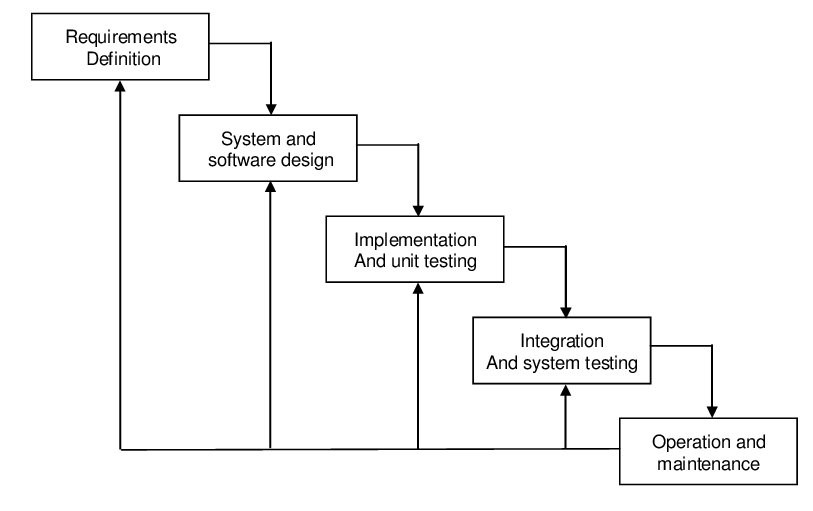
\includegraphics[width=15cm]{wf.png}
		\end{center}
		In “The Waterfall” approach, the whole process of software development is divided into separate phases. The outcome of one phase acts as the input for the next phase sequentially. This means that any phase in the development process begins only if the previous phase is complete. The waterfall model is a sequential design process in which progress is seen as flowing steadily downwards (like a waterfall) through the phases of Conception, Initiation, Analysis, Design, Construction, Testing, Production/Implementation, and Maintenance.
		\vs
		As the Waterfall Model illustrates the software development process in a linear sequential flow; hence it is also referred to as a \textbf{\em Linear-Sequential Life Cycle Model}.
		\subsection{Sequential Phases in the Waterfall Model}
		\begin{itemize}
			\item
			\textbf{\large Requirements}
			
			The first phase involves understanding what needs to design and what is its function, purpose, etc. Here, the specifications of the input and output or the final product are studied and marked.
			\item
			\textbf{\large System Design}
			
			The requirement specifications from the first phase are studied in this phase and system design is prepared. System Design helps in specifying hardware and system requirements and also helps in defining overall system architecture. The software code to be written in the next stage is created now.
			\item
			\textbf{\large Implementation}
			
			With inputs from system design, the system is first developed in small programs called units, which are integrated into the next phase. Each unit is developed and tested for its functionality which is referred to as Unit Testing.
			\item
			\textbf{\large Integration and Testing}
			
			All the units developed in the implementation phase are integrated into a system after testing of each unit. The software designed, needs to go through constant software testing to find out if there are any flaws or errors. Testing is done so that the client does not face any problem during the installation of the software.
			\item
			\textbf{\large Deployment of System}
			
			Once the functional and non-functional testing is done, the product is deployed in the customer environment or released into the market.
			\item
			\textbf{\large Maintenance}
			
			This step occurs after installation, and involves making modifications to the system or an individual component to alter attributes or improve performance. These modifications arise either due to change requests initiated by the customer, or defects uncovered during live use of the system. The client is provided with regular maintenance and support for the developed software.
		\end{itemize}